\input{../preamble.tex}

\lecturenumber{19}
\title{Threads}
\version{2.0.0}

\begin{document}
	\begin{frame}[plain, noframenumbering]
		\titlepage
	\end{frame}

	\begin{slide}
	
		\slidetitle{Mid-Semester Re-cap}
	
	    \begin{center}
        \begin{tabular}{  l l l l  } 
          \textbf{Assessment} & \textbf{Weight} & \textbf{Status} \\ 
          Lab 1 & 7.5\% & Completed \\ 
          Midterm & 20\% & Completed \\ 
          Lab 2 & 7.5\% & Completed \\ 
          Lab 3 & 7.5\% &   \\ 
          Lab 4 & 7.5\% &   \\ 
          Final & 50\% &  \\ 
        \end{tabular}
    \end{center}
	
	\end{slide}
	
	\begin{slide}
	
		\slidetitle{Course Topics}
		
		OS Fundamentals
		\medskip
		
		Process
		\medskip
		
		Scheduling
		\medskip
		
		Memory
		\bigskip
		
		Concurrency
		\medskip
		
		File Systems
		\medskip
		
		Security, Device Drivers
		
	
	\end{slide}
	
	\begin{slide}
	
		\slidetitle{Information on Final Exam}
		
		June 23rd, 2 pm, 2 hrs 15 mins
		
		\bigskip
		
		Openbook, No calculators permitted
		
		\bigskip
		
		Format: 50 Multiple-choice (tentative)
	
		\bigskip
		
		About 15 questions on the 1st half of the course, 35 questions on the 2nd half
		
	\end{slide}
	
	\begin{slide}
	
		\slidetitle{Plans This Week}
	
		Collect your teleform sheets.
		\bigskip
		
		Tutorial: Midterm Questions
		
	\end{slide}
	
	
	\begin{slide}
	
		\slidetitle{Concurrency: Multi-thread Programming}
		
		Game programming: The main thread renders each frame, while a pool of worker threads processes gameplay tasks (AI, physics, audio) in parallel.
		
		\bigskip
		
		Machine learning: Training launches thousands of lightweight GPU threads per kernel.
		
		\bigskip
		
		Web programming: Server thread pools handle large numbers of concurrent HTTP requests, overlapping I/O and computation to maximize throughput.
	
	\end{slide}
	
	\begin{slide}
	
		\slidetitle{Throwback: Process and \texttt{fork()}}
		
		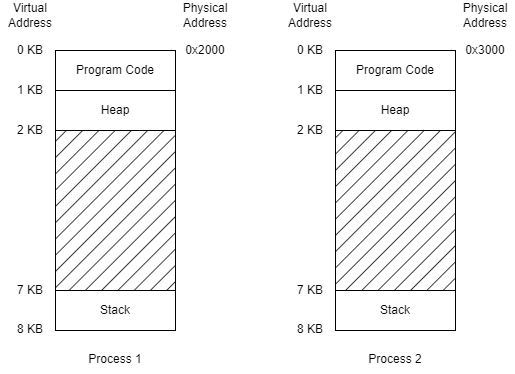
\includegraphics[width=80mm]{multi-process-memory.png}
		
	\end{slide}

	\begin{slide}
	
		\slidetitle{Multi-Thread Memory}
		
		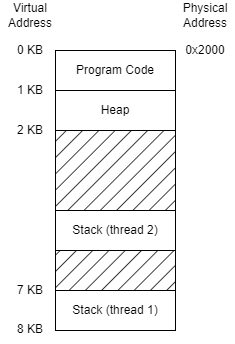
\includegraphics[width=30mm]{multi-thread-memory.png}
		
		\medskip
		
		What are the trade-offs?
		
	\end{slide}
	
 
	\begin{slide}

		\slidetitle{Threads are Like Processes with Shared Memory}

		The same principle as a process, except by default they share memory

		\leftspace{}They have their own registers, program counter, and stack
		\medskip

		They have the same address space, so changes appear in each thread
		\medskip

		You need to explicitly state if any memory is specific to a thread (TLS)

	\end{slide}

	\begin{slide}

		\slidetitle{One Process Can have Multiple Threads}

		By default, a process just executes code in its own address space
		\medskip

		Threads allow multiple executions in the same address space
		\medskip

		They're lighter weight and less expensive to create than processes

		\leftspace{}They share code, data, file descriptors, etc.

	\end{slide}

	\begin{slide}

		\slidetitle{Aside: Concurrency and Parallelism Aren't the Same}

		Concurrency

		\leftspace{}Switching between two or more things (can you get interrupted)

		\leftspace{}\leftspace{}Goal: make progress on multiple things
		\bigskip

		Parallelism

		\leftspace{}Running two or more things at the same time (are they independent)

		\leftspace{}\leftspace{}Goal: run as fast as possible
		\bigskip
		
		Multi-thread programming can achieve both.
		
	 \end{slide}
  
   \begin{slide}

		\slidetitle{We'll be Using POSIX Threads}

		For Windows, there's a Win32 thread, but we're going to use *UNIX threads
		\medskip

		\mintinline{c}{#include <pthread.h>} --- in your source file
		\medskip

		\mintinline{c}{-pthread} --- compile and link the pthread library
		\medskip

		All the pthread functions have documentation in the \mintinline{c}{man} pages

   \end{slide}

  \begin{slide}

    \slidetitle{You Create Threads with \texttt{pthread\_create}}

    \begin{minted}{c}
int pthread_create(pthread_t* thread, 
                   const pthread_attr_t* attr,
                   void* (*start_routine)(void*),
                   void* arg);
    \end{minted}
    \medskip

    \begin{tabular}{rl}
      thread & creates a handle to a thread at pointer location \\

      attr & thread attributes (NULL for defaults, more details later) \\

      start\_routine & function to start execution \\

      arg & value to pass to start\_routine \\
    \end{tabular}

    returns 0 on success, error number otherwise
    
    \leftspace{}(contents of *thread are undefined)

  \end{slide}

  \begin{slide}

    \slidetitle{Creating a thread}

	\vspace{-5mm}
	
    \begin{minted}{c}
#include <pthread.h>
#include <stdio.h>

void* run(void *arg) {
  printf("%s\n", (char *) arg);
  return NULL;
}

int main() {
  pthread_t p1, p2;
  pthread_create(&p1, NULL, &run, "A");
  pthread_create(&p2, NULL, &run, "B");
  printf("In main\n");
}
    \end{minted}

  \end{slide}

  \begin{slide}

    \slidetitle{The \texttt{wait} Equivalent for Threads --- Join}

    \begin{minted}{c}
int pthread_join(pthread_t thread,
                 void** retval)
    \end{minted}
    \medskip

    \begin{tabular}{rp{10cm}}
  thread & wait for this thread to terminate (thread must be joinable) \\

  retval & stores exit status of thread (set by {\tt pthread\_exit}) to
                 the location pointed by *retval. If cancelled returns
                 {\tt PTHREAD\_CANCELED}. {\tt NULL} is ignored. \\
    \end{tabular}

  returns 0 on success, error number otherwise 
  \medskip

  {\bf Only call this one time per thread!}

  \leftspace{}Multiple calls on the same thread leads to undefined behavior

  \end{slide}

	\begin{slide}

		\slidetitle{Previous Example that Waits Properly}

		\vspace{-5mm}
		
		\begin{minted}{c}
void* run(void *arg) {
  printf("%s\n", (char *) arg);
  return NULL;
}

int main() {
  pthread_t p1, p2;
  pthread_create(&p1, NULL, &run, "A");
  pthread_create(&p2, NULL, &run, "B");
  pthread_join(p1, NULL);
  pthread_join(p2, NULL);
  printf("In main\n");
}
		\end{minted}

	\end{slide}
	
	\begin{slide}
	
		\slidetitle{Recap for Yesterday}
		
	Threads are like processes with shared memory.
	\bigskip
	
	Creating a thread:
	\begin{minted}{c}
int pthread_create(pthread_t* thread, 
                   const pthread_attr_t* attr,
                   void* (*start_routine)(void*),
                   void* arg);
    \end{minted}
    \bigskip
		
	Waiting on a thread to finish:
	\begin{minted}{c}
int pthread_join(pthread_t thread,
                 void** retval)
    \end{minted}
    \medskip
	
	\end{slide}
	
	\begin{slide}
	
		\slidetitle{An Array Example}
		
		I want to create a 1\(\times\)5 \texttt{int} array and fill it with the elements 
		
		\leftspace \{10, 20, 30, 40, 50\}.
		\medskip
		
		I want to create a thread to handle this task.
		\bigskip
		
		Where do I allocate this memory?
		\bigskip
		
		Which thread allocates the memory?
		
	\end{slide}
	
	\begin{slide}
	
		\slidetitle{An Array Example - Main Thread Allocates}
		\vspace{-4mm}
	\begin{minted}{c}
#define N 5
void *array_ex(void *arg)
{
    int *a = arg;                
    for (int i = 0; i < N; ++i)
        a[i] = (i + 1) * 10;     
    return NULL;               
}
int main(void)
{
    pthread_t p1;
    int *array = malloc(N * sizeof(int);
    thread_create(&p1, NULL, array_ex, array);
    pthread_join(p1, NULL);
    free(array);
    return 0;
}
	\end{minted}
	
	\end{slide}
	
		\begin{slide}
	
		\slidetitle{An Array Example - Worker Thread Allocates}
		\vspace{-4mm}
	\begin{minted}{c}
#define N 5
void *make_array(void *arg)
{
    int *a = malloc(N * sizeof(int));
    for (int i = 0; i < N; ++i)
        a[i] = (i + 1) * 10;          
    return a;                       
}
int main(void)
{
    pthread_t tid;
    int *array = NULL;
    pthread_create(&tid, NULL, make_array, NULL) != 0;
    pthread_join(tid, (void **)&array);
    free(array);                     
    return 0;
}
	\end{minted}
	
	\end{slide}
	
		\begin{slide}

		\slidetitle{Previous Example that Waits Properly}

		\vspace{-5mm}
		
		\begin{minted}{c}
void* run(void *arg) {
  int* retval = malloc(sizeof(int));
  *retval = 42;
  return retval;
}
int main() {
  pthread_t p1;
  void* ret_val;
  
  pthread_create(&p1, NULL, &run, "A");
  pthread_join(p1, &ret_val);
 
  int result = *(int*)ret_val;
  free(ret_val);
}
		\end{minted}

	\end{slide}

	\begin{slide}

		\slidetitle{Ending a Thread Early (Think of \texttt{exit})}

		\begin{minted}{c}
void pthread_exit(void *retval);
		\end{minted}
		\medskip

		\begin{tabular}{rl}
		  retval & return value passed to function that calls {\tt pthread\_join} \\
		\end{tabular}
		\medskip
		
		Note: \mintinline{c}{start_routine} returning is equivalent of calling {\tt pthread\_exit}

		\leftspace{}Think of the difference between returning from main and
		\texttt{exit}
		\medskip

		{\tt pthread\_exit} is called implicitly when the {\tt start\_routine} of a
		thread returns

	\end{slide}
	
	
		\begin{slide}

		\slidetitle{Previous Example that Waits Properly}

		\vspace{-5mm}
		
		\begin{minted}{c}
void* run(void *arg) {
  int* retval = malloc(sizeof(int));
  *retval = 42;
  return retval; // pthread_exit(retval) is called;
}
int main() {
  pthread_t p1;
  void* ret_val;
  
  pthread_create(&p1, NULL, &run, "A");
  pthread_join(p1, &ret_val);
 
  int result = *(int*)ret_val;
  free(ret_val);
}
		\end{minted}

	\end{slide}
	
  \begin{slide}

		\slidetitle{Detached Threads}

		{\it Joinable} threads (the default) wait for someone to call
		{\tt pthread\_join}

		\leftspace{}then they release their resources
		\medskip

		{\it Detached} threads release their resources when they terminate
		\medskip

		\begin{minted}{c}
int pthread_detach(pthread_t thread);
		\end{minted}
		\medskip

		\begin{tabular}{rl}
		  thread & marks the thread as detached \\
		\end{tabular}

		returns 0 on success, error number otherwise
		\medskip

		Calling {\tt pthread\_detach} on an already detached is undefined
		behavior

	\end{slide}

	\begin{slide}

		\slidetitle{Detached Threads Aren't Joined}

		\begin{minted}{c}
void* run(void*) {
  printf("In run\n");
  return NULL;
}

int main() {
  pthread_t thread;
  pthread_create(&thread, NULL, &run, NULL);
  pthread_detach(thread);
  printf("In main\n");
  return 0;
}
		\end{minted}
		\medskip

		This code just prints ``In main'', why?

	\end{slide}

	\begin{slide}

		\slidetitle{\texttt{pthread\_exit} in main Waits for All Detached Threads to Finish}

		\begin{minted}{c}
void* run(void*) {
  printf("In run\n");
  return NULL;
}

int main() {
  pthread_t thread;
  pthread_create(&thread, NULL, &run, NULL);
  pthread_detach(thread);
  printf("In main\n");
  pthread_exit(NULL);
}
		\end{minted}
		\medskip

	\end{slide}

	\begin{slide}

		\slidetitle{You Can Use Attributes To Get/Set Thread Variables}

		\begin{minted}{c}
size_t stacksize;
pthread_attr_t attributes;
pthread_attr_init(&attributes);
pthread_attr_getstacksize(&attributes, &stacksize);
printf("Stack size = %i\n", stacksize);
pthread_attr_destroy(&attributes);
		\end{minted}

		Running this should show a stack size of 8 MiB (on most Linux systems)

	\end{slide}

  \begin{slide}

    \slidetitle{Multithreading Models}

    Where do we implement threads?

    \leftspace{}We can either do user or kernel threads
    \medskip

    User threads are completely in user-space

    \leftspace{}Kernel doesn't treat your threaded process any differently
    \medskip

    Kernel threads are implemented in kernel-space

    \leftspace{}Kernel manages everything for you, and can treat threads specially

  \end{slide}

  \begin{slide}
    \slidetitle{Thread Support Requires a Thread Table}

    Similar to the process table we saw previously
    
    \leftspace{}It could be in user-space or kernel-space (depending)
    \medskip

    For user threads, there also needs to be a run-time system to determine
    scheduling
    \medskip

    In both models each process can contain multiple threads

  \end{slide}

  \begin{slide}

    \slidetitle{We Could Avoid System Calls, or Let a Thread Block Everything}

    For pure user-level threads (again, no kernel support):

    \begin{itemize}
      \item Very fast to create and destroy, no system call, no context switches
      \item One thread blocks, it blocks the entire process (kernel can't distinguish)
    \end{itemize}
    \medskip

    For kernel-level threads:

    \begin{itemize}
      \item Slower, creation involves system calls
      \item If one thread blocks, the kernel can schedule another one
    \end{itemize}

  \end{slide}

  \begin{slide}

    \slidetitle{All Threading Libraries You Use Run in User-mode}

    The thread library maps user threads to kernel threads
    \medskip

    Many-to-one: threads completely implemented in user-space

    \leftspace{}the kernel only sees one process
    \medskip

    One-to-one: one user thread maps directly to one kernel thread

    \leftspace{}the kernel handles everything
    \medskip

    Many-to-many: many user-level threads map to many kernel level threads

  \end{slide}

  \begin{slide}

    \slidetitle{Many-to-one is Pure User-space Implementation}

    It's fast (as outlined before) and portable

    \leftspace{}It doesn't depend on the system, it's just a library
    \medskip

    Drawbacks are that one thread blocking causes all threads to block

    \leftspace{}Also, we cannot execute threads in parallel

    \leftspace{}\leftspace{}The kernel will only schedule a process to run

  \end{slide}

  \begin{slide}

    \slidetitle{One-to-one Just Uses the Kernel Thread Implementation}

    There's just a thin wrapper around the system calls to make it easier to use
    \medskip

    Exploits the full parallelism of your machine

    \leftspace{}The kernel can schedule multiple threads simultaneously
    \medskip

    We do however need to use a slower system call interface,

    \leftspace{}and we lose some control
    \bigskip

    Typically, this is the actual implementation used, we'll assume this for
    Linux

  \end{slide}

  \begin{slide}

    \slidetitle{Many-to-many is a Hybrid Approach}

    The idea is that there are more user-level threads than kernel-level threads

    \leftspace{}Cap the number of kernel-level threads to the number we could
    run in parallel
    \medskip

    We can get the most out of multiple CPUs and reduce the number of system
    calls
    \medskip

    However, this leads to a complicated thread library (Java Virtual Threads)

    \leftspace{}Depending on your mapping luck, you may block other threads

  \end{slide}

  \begin{slide}

    \slidetitle{Threads Complicate the Kernel}

    How should \texttt{fork} work with a process with multiple threads?

    \leftspace{}Copy all threads to the new process, in whatever state they're
    in?

    \leftspace{}\leftspace{}How would this get out of hand?
    \medskip

    Linux only copies the thread that called \texttt{fork} into a new process

    \leftspace{}If it hits \texttt{pthread\_exit} it'll always exit with
                  status 0

    \leftspace{}\leftspace{}(at least as far as I can tell)
    \medskip

    There's \texttt{pthread\_atfork} (not covered in this course) to control
    what happens

  \end{slide}

  \begin{slide}

    \slidetitle{Signals are Sent to a Process}

    Which thread should receive a signal? all of them?
    \medskip

    Linux will just pick one random thread to handle the signal

    \leftspace{}Makes concurrency hard, any thread could be interrupted

  \end{slide}

  \begin{slide}

    \slidetitle{Instead of Many-to-many, You Can Use a Thread Pool}

    The goal of many-to-many thread mapping is to avoid creation costs
    \medskip

    A thread pool creates a certain number of threads and a queue of tasks

    \leftspace{}(maybe as many threads as CPUs in the system)
    \medskip

    As requests come in, wake them up and give them work to do
    \medskip

    Reuse them, when there's no work, put them to sleep

  \end{slide}


\end{document}
